\chapter{XML Modeling Extension} \label{ch:xmlparser}

Modeling complex human-machine systems is a very difficult and time-consuming task.  This is evidenced by an abundance of modeling approaches for systems involving humans (ACT-R~\cite{anderson1996act}, Soar~\cite{laird2012soar}, DIARC~\cite{schermerhorn2006diarc}, Brahms~\cite{clancey1998brahms}, EOFM~\cite{bolton2009enhanced}), the panel ``Modeling Hurts'' AAAI workshop on Formal Methods in Human-Machine Systems~\cite{aaaisymposium2014modeling}, and our own experiences in generating the WiSAR models.

By constructing the Modeling Interface aspect of the Model Abstraction Framework as a set of Java interfaces and abstract classes it meant that the framework was extremely flexible.  This approach enforces only a minimum set of requirements at the model level.  While this is very powerful it relies on the modeler for all requirements that cannot be enforced by the interfaces.  In our initial model we found implicit declarations, inconsistencies, duplicated code, coding bugs, and anonymous methods (unbound functions with access to local scope that can be declared in-line and make debugging and readability more difficult).  Each of these artifacts degrades the usability, extensibility, and maintainability of the model.  More importantly, it becomes almost impossible to know if the models are valid and error-free, which directly affects metric validity.  This chapter discusses an approach to creating Model Abstraction Framework models that reduce modeling issues while simplifying the modeling process.

\section{Modeling Approach}

One approach for improving modeling efficiency is to create GUIs that help the user visualize the model in a way that allows them to more easily understand and make changes to the model.  An example of this is the Brahms Composer~\cite{seah2005multi}, which allows the user to create models on the GUI and to visualize the model in different ways.  Another approach is to use a language structure that is human readable and facilitates the creation of an accurate mental model.  An example of this is EOFM~\cite{bolton2009enhanced}, which uses an XML structure that can be visualized as a tree graph.  The last approach we will mention is the use of design patterns and object oriented principles to build models that do not exhibit these problems.  The downside to this approach is it requires expert Java programming skills to build error-free models.

While others have successfully taken the third approach, for this thesis we chose to take an approach similar to that of EOFM by constructing an XML structure to represent our labeled state transition system.  Unlike EOFM, the XML structure is not the main modeling language.  The XML structure represents the subset of the Model Abstraction Framework language that is represented by the underlying Java objects implementing the Modeling Interface.  We chose this approach for several reasons:  XML is commonly used for modeling and other similar tasks~\cite{bolton2009enhanced}, it is simple to work with in Java, it is human readable, and it is structured.  This gave us confidence that we would be able to generate an XML model, perform validation on the model, and then convert the model into Java.  We also chose this approach because XML is semantically constrained to the structure we define.  The modeler needs only a basic understanding of XML structures and the defined modeling semantics to implement a model.  Another reason for this approach is the consistency with the Model Abstraction Framework design.  The Model Abstraction Framework represents a top down approach to abstraction, meaning that the top level Actors, States, Transitions, and Channels are very abstract.  Each subsequent layer removes a portion of that abstraction.  The XML modeling extension adds constraints to the top level Modeling Interface that are designed to remove unnecessary modeling capabilities from the modeling language.

\section{XML Structure}

We defined the following XML structure to represent the labeled state transition system sent to the simulator.  

The root node is the {\em \textless team\textgreater} element which consists of the {\em name} attribute and three child elements: {\em \textless channels\textgreater}, {\em \textless actors\textgreater}, and {\em \textless events\textgreater}.

\begin{spacing}{.5}
\lstinputlisting[language=XML]{xml_team.xml}
\end{spacing}

\subsection{Channels}

The {\em \textless channels\textgreater} element represents the DiTG and is comprised of any number of {\em \textless channel\textgreater} elements.  Each {\em \textless channel\textgreater} element represents a single uni-directional communication channel between a source Actor and a target Actor with attributes for the name, type, source, target, and optional dataType.  This is the only location in the XML that defines channels.  Every other {\em \textless channel\textgreater} element references one of these channels by using the channel name as its value.  In future work, we hope to identify other properties of channels such as bandwidth.

\begin{spacing}{.5}
\lstinputlisting[language=XML]{xml_channels.xml}
\end{spacing}

\subsection{Actors}

The {\em \textless actors\textgreater} element represents the DiRGs contained in the model and is comprised of one or more {\em \textless actor\textgreater} elements.  Each {\em \textless actor\textgreater} has a {\em name} attribute, which must be unique, and a {\em showMetrics} attribute and is made up of several child elements.  The {\em \textless inputchannels\textgreater} and {\em \textless outputchannels\textgreater} elements are placed here to validate the DiTG.  The {\em actor} may have zero or more {\em memory} elements that represent declarative memory, memory that is an active part of the cognitive decision process, and is used internally as part of the labeled state transitions.  The {\em \textless actor\textgreater} contains a list of one or more {\em \textless state\textgreater} elements inside of the {\em \textless states\textgreater} element.  Additionally the {\em \textless actor\textgreater} element must contain a single {\em \textless startState\textgreater} element with a value that matches the name attribute of one of the {\em \textless states\textgreater} child elements.

\begin{spacing}{.5}
\lstinputlisting[language=XML]{xml_actors.xml}
\end{spacing}


\subsection{States and Transitions}

The {\em \textless state\textgreater} element represents the `State' in the labeled state transition system.  Each {\em \textless state\textgreater} element has a {\em name} attribute, which must be unique to the parent {\em \textless actor\textgreater} element, and a {\em load} attribute with a value of 0-4 (we will discuss state load in the next chapter).  The {\em \textless state\textgreater} element also contains zero or more {\em \textless transition\textgreater} child elements.  If no {\em \textless transition\textgreater} child elements are specified then it is an end state.  

The {\em \textless transition\textgreater} element represents the `Transition' in the labeled state transition system and is composed of {\em durationMin} and {\em durationMax} attributes that are used to create a transition duration range to enable timing analysis in JPF.  It also has a {\em priority} attribute used to rank a transitions priority with respect to the other state transitions.  Each {\em \textless transition\textgreater} element contains four child elements: {\em \textless description\textgreater}, {\em \textless inputs\textgreater}, {\em \textless outputs\textgreater}, and {\em \textless endState\textgreater}.  

The {\em \textless description\textgreater} element value contains a description of the transition that is meant to help give the modeler insight into what the transition is actually doing.  It is also used in the debug logs to help track down modeling errors.  

The {\em \textless inputs\textgreater} and {\em \textless outputs\textgreater} elements represent the `Label' in the labeled state transition system.  These elements contain zero or more {\em \textless memory\textgreater} and {\em \textless channel\textgreater} elements.  All {\em \textless inputs\textgreater} element children have a {\em name} attribute, a {\em predicate} attribute, an optional {\em dataType} attribute and a value.  If the child element is a {\em \textless channel\textgreater} then it may optionally declare only the {\em name} attribute and one or more {\em \textless layer\textgreater} child elements to specifically describe the different types of data being sent over the channel.  The {\em \textless layer\textgreater} element consists of {\em name}, {\em predicate}, and optional {\em dataType} attributes with an accompanying data value.  The {\em \textless channel\textgreater} name must correlate with an {\em \textless actor\textgreater} {\em \textless inputchannels\textgreater} {\em \textless channel\textgreater} value.  The {\em predicate} attribute contains one of six predicate values: equal to, not equal, greater than, less than, greater than or equal, or less than or equal.  The {\em dataType} is one of three options: String, Integer, or Boolean with a default of String.  The value of these child elements is the value that will be compared against the channel or memory value.  

The {\em \textless outputs\textgreater} element is similar to the {\em \textless inputs\textgreater} element except that its children do not specify {\em predicate} or {\em dataType} attributes.  

This structure allows the modeler to use a 2 dimensional labeling system.  The first dimension is the direction of the data flow, input or output.  The second dimension is the source of the data; channel, layer, or memory.  This allows the labeled state transition system to be very flexible while using a relatively simple syntax.  We should also point out that the transition {\em \textless inputs\textgreater} element uses the following propositional logic: $(Child_{1} \bigwedge Child_{2} \bigwedge \ldots \bigwedge Child_{n})$.  This means that all transition inputs are evaluated together, preventing the modeler from defining multiple sets of inputs for a single transition.  Thus each labeled state transition, no matter how similar to another, must be expressed as a separate {\em \textless transition\textgreater} element.

The value of the {\em \textless endState\textgreater} element contains the name of the Actor's ending state if this transition is applied.  This value cannot be empty and must match an existing {\em \textless state\textgreater} name.

\begin{spacing}{.5}
\lstinputlisting[language=XML]{xml_state_transition.xml}
\end{spacing}


\subsection{Events}

The {\em \textless events\textgreater} element contains a child {\em \textless event\textgreater} element for each unique type of event the system can experience.  The {\em \textless event\textgreater} has a {\em name} attribute, must be unique, and a {\em count} attribute that determines how many times the event will be fired during the simulation.  Each {\em \textless event\textgreater} element defines a single {\em \textless transition\textgreater} element that differs from the previously mentioned transition element in that it does not define duration, priority, or an end state.  Since Events have a single state and a single transition there is no need for these additional transition attributes.  At the implementation level this forces Events to act as sipmle triggers that perturb the model in interesting ways.

\begin{spacing}{.5}
\lstinputlisting[language=XML]{xml_events.xml}
\end{spacing}

\section{XML Model Parser}

Figure~\ref{fig:xml_model_extension} illustrates the process of parsing the XML model.  To accomplish this we created a Java class named XMLModelParser.  This class performed two main functions.  The first was to create the necessary Java objects and the second was to perform basic error checking on the model.  

The XMLModelParser works by first loading the XML model into an XML object.  This allows us to search the XML structure for specific elements and attributes.  The structure of the XML model facilitates the parsing effort since each child element is also a child object.  The first object that is created is the Team.  Next the DiTG is added to the team by creating ComChannel objects for each channel.  The Actor parsing is the most complex.  Each actor element defines input and output channels, memory, states, transitions, and labels.

\begin{figure}[h]
\begin{center}
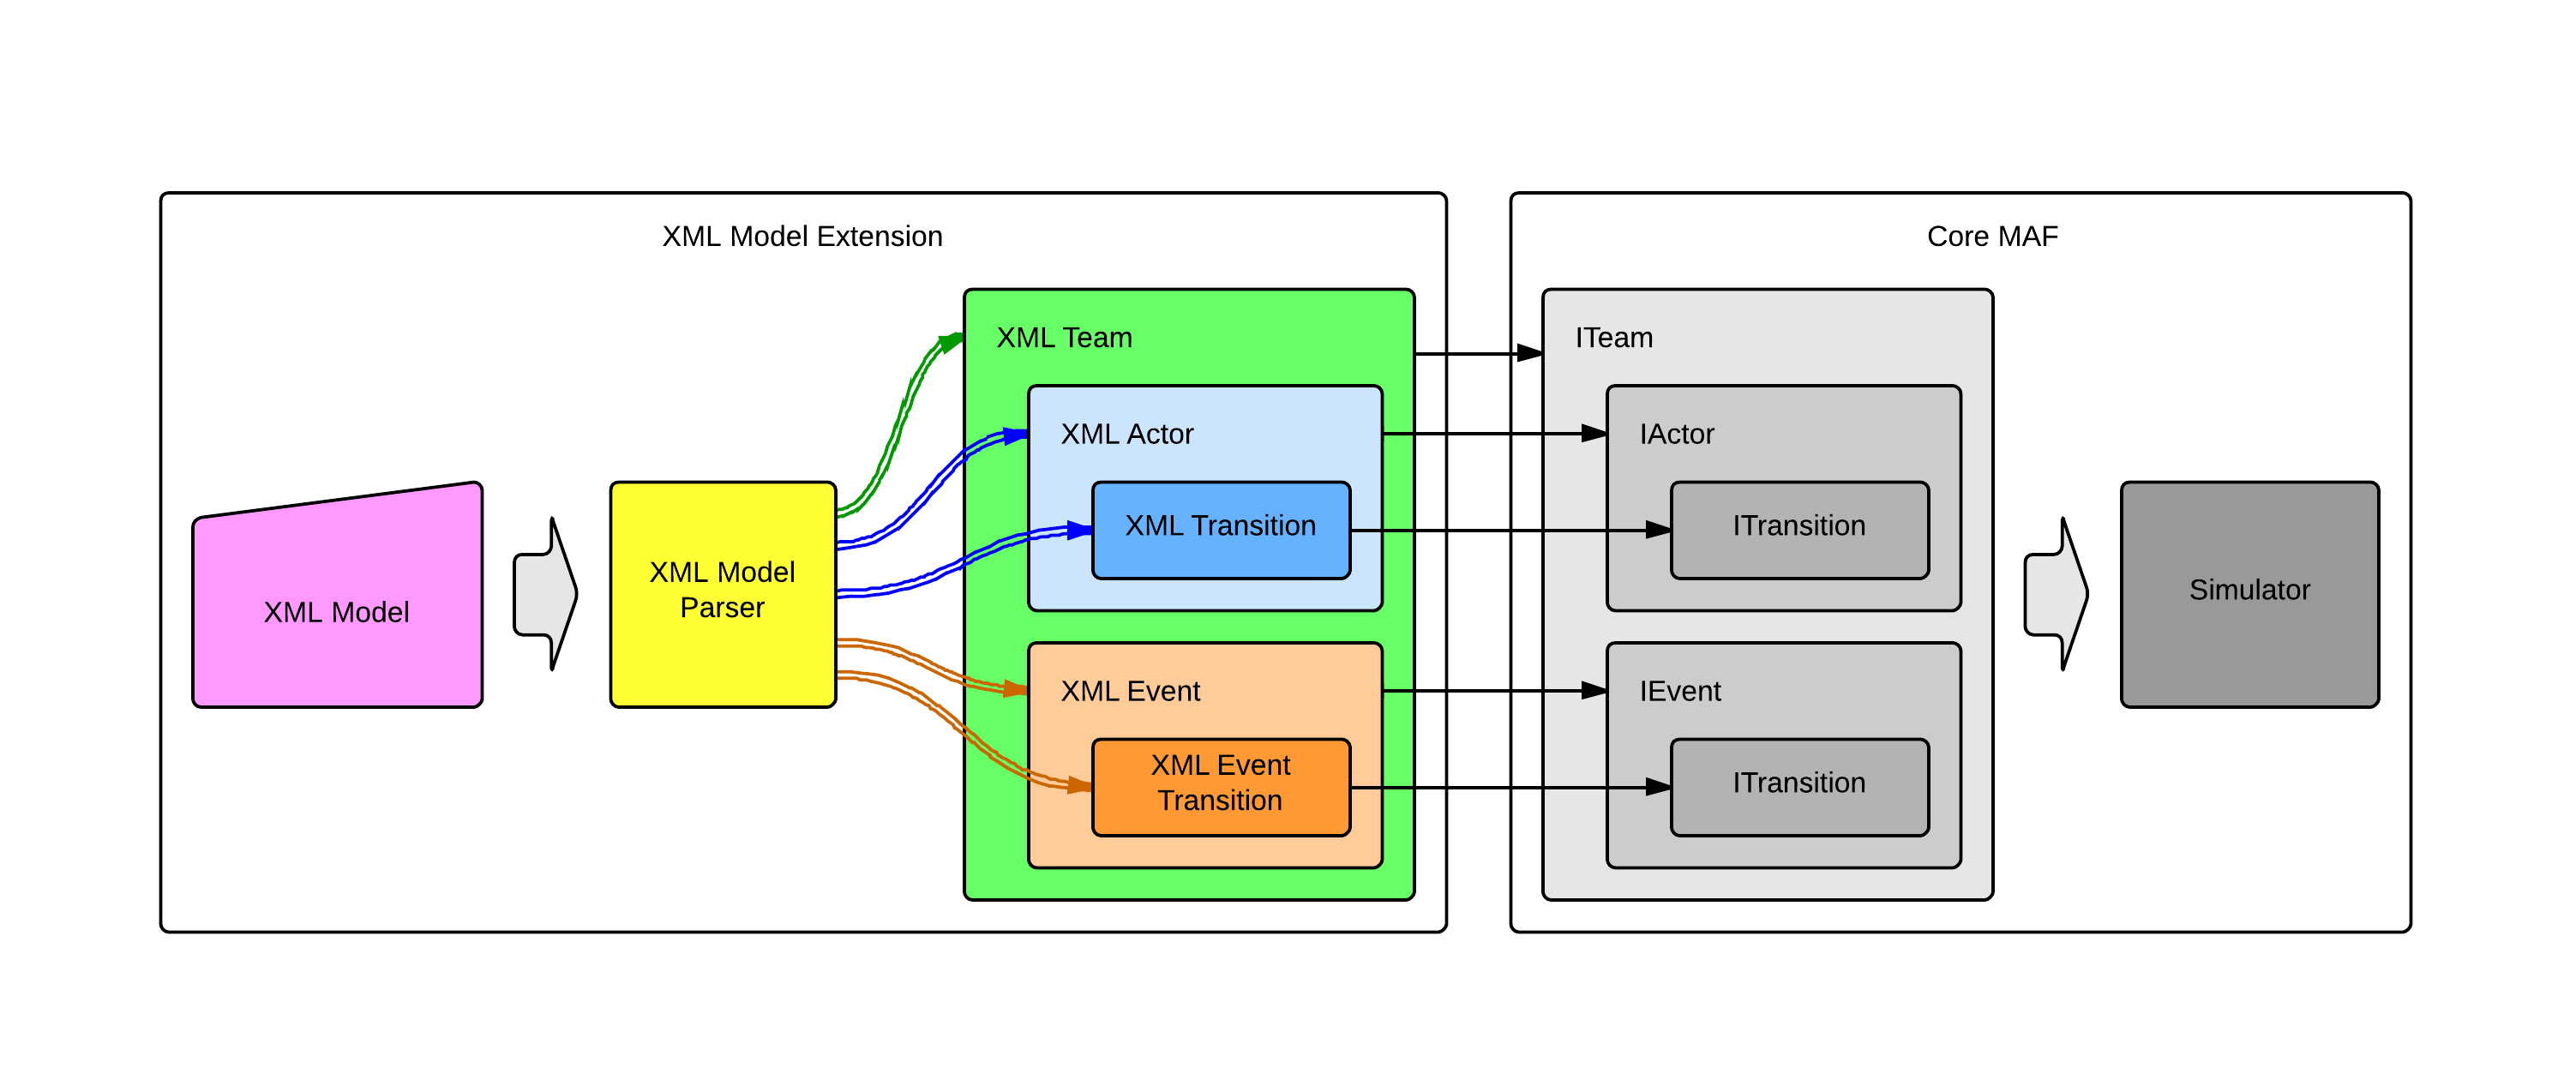
\includegraphics[width=\textwidth]{xml_model_extension.png}
\caption{XML Model Extension Breakdown}
\label{fig:xml_model_extension}
\end{center}
\end{figure}

\subsection{Attaching to the Simulator}

To pass a valid labeled state transition system to the simulator, the XMLModelParser must construct Java classes that implement the Modeling Interface.  To accomplish this we created a set of generic XML classes.  Each class implements a specific portion of the Modeling Interface such as the ITransition or IActor interfaces.  These interfaces allow the simulator to query and execute transitions on the labeled state transition system.  The list of XML classes includes the XMLTeam, XMLActor, XMLTransition, XMLEvent, XMLEventTransition and other helper classes.  A link to the source code can be found in appendix~\ref{code}.  Each of these generic XML classes lies separate from the core simulation code.  

This means that the addition of the XML parser does not prevent the use of custom Actors or Transition classes, use of a different model parser, or extension of our existing XML parser.  In fact our XML model extension is meant to be expanded to handle a more robust set of models.   As we developed a model using this XMLModelParser we had several occasions to extend its capabilities, which we discuss later.  Unsurprisingly it was not difficult to extend the XML to accommodate the changes, often requiring less than 100 lines of code (not including changes to the model XML).

\subsection{Validation}

Model validation occurred in three phases: Sample WiSAR, Full WiSAR, and UAS in NAS\footnote{Jared Moore and Robert Ivie were a great help in constructing, validating, and running the Sample WiSAR and Full WiSAR models.  Without their excellent contributions this work would have taken much longer to complete.}.  In each phase a model was created and validated.  The models from the first two phases were written in Java and directly implemented the Modeling Interface.  The UAS in NAS model was written in XML using the XML Modeling Extension.  This section discusses the challenges we observed during the first two modeling phases, and compares those results against the last modeling phase.

\begin{figure}[h]
\begin{center}
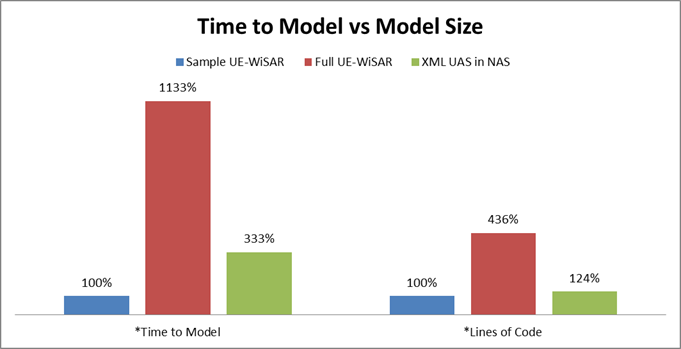
\includegraphics[width=5in]{time_to_model.png}
\caption{Time to Model vs Model Size}
\label{fig:time_to_model}
\end{center}
\end{figure}

One of the most time consuming aspect of the modeling process was validating that the model was correct.  By correct we mean that each designed path through the model can and will be traversed when given a specific set of inputs.  In order to ensure that the model was correct we had to manually step through the model simulation paths during construction and check that the correct paths were being taken.  While this was a simple task in the Sample WiSAR phase it was much more challenging during the Full WiSAR modeling phase.  According to commit dates in our github repository we estimate that the Sample WiSAR model, containing 5 Actors, took three days to create and validate.  The following 12 Actor Full WiSAR model took 34 days to create and validate.  However, the fully functional model only contained four times the amount of code.  Figure~\ref{fig:time_to_model}~\footnote{In figure~\ref{fig:time_to_model} time to model is an approximation generated by analyzing github commits.  Also lines of code has been adjusted to account for whitespace, comments, and lines with fewer than 5 characters.}.  The discrepancy between the time to model and the model size demonstrates how problematic model validation can become as model complexity increases.

During the Full WiSAR modeling phase we observed several underlying modeling problems that we believe are responsible for the dramatic increase in validation time.  The first problem occurred when the modeler became disoriented while working within the model.  Each time a path branches or the modeler switches branches it becomes more likely that their mental model will diverge from the Java model.  As complexity increases the number of branches and the need to jump between branches also increases.  When this happens, mistakes related to a divergent mental model, such as transitioning to the wrong state, forgetting to add a transition, or checking the wrong inputs, begin to appear.  Another problem was a lack of validation tools.  The step-through validation approach essentially meant that only a single modeling error could be found at a time and we had to step through the entire model for each error.  We also observed that modelers are prone to introduce common typing errors into the model that do not get caught by the Java compiler.  

During the UAS in NAS phase the XML Modeling Extension helped to mitigate these problems in a few different ways.  The XML modeling structure offsets some of the complexity by presenting the model to the user in a more compact and semantically relevant form.  Java syntax such as class, new, void, etc. are not relevant to the model and do not help the modeler understand the model.  The XML specific syntax, however, uses a much smaller footprint.  Additionally the structure itself describes the model in a very concise form that helps the modeler maintain a more accurate mental model leading to fewer modeling errors.

This extension also helps by introducing a new validation tool.  The need to parse the XML into Java provides a natural location to perform basic error checking on the XML before creating the Java objects that are passed to the simulator. The simple syntax and structure of the XML makes it much easier to check for user errors in the model.  One of the most common errors we found when creating the UAS in NAS model was missing parameters.  Inside the XMLModelParser, if a required portion of XML is not found an error is returned with a description of the problem and where it occurred.  The same is true for an invalid DiTG, duplicate element names, typos, and missing or impossible transitions.  This provided huge time savings when compared with the other alternatives of analyzing output logs or stepping through code with the debugger.

Another benefit introduced with this extension was the generic Java classes.  Each XML component had a single Java implementation.  This guaranteed that similar components would share the same behavior, something that Java interfaces do not provide.  It also meant that bugs in the Java code only needed to be fixed in a single location.

\section{Channel Layers}

While working on this extension it became apparent that our channel design was flawed.  From Threaded Cognition Theory~\cite{salvucci2008threaded} we are aware that an individual can perform multiple concurrent tasks that do not require an executive process.  It does not matter if those concurrent tasks originate from multiple sources or a single source, such as a GUI.  Our previous design restricted channels to a single type of data with no restriction as to what that data type was.  While an arbitrary data type allowed us to pass any amount of data, it made it very difficult to know what was really happening on the communication channel.  What we mean by this is that instead of explicitly defining concurrent tasks we rely on inputs and actor state to imply that concurrent tasks are being performed.  The arbitrary data type thus prevented a single communication channel from implying multiple concurrent tasks.

To fix this flaw we decided to add layers to our communication channels. Figure~\ref{fig:layers}.  Each channel can have any number of layers.  For example, a visual channel from one person to another has two channels, one that analyzes the face and another that analyzes the body.  There may be more accurate channel layering for this scenario but these layers satisfy this example.  When communication occurs on this visual channel the recipient can examine as many layers as are needed for the given state.  If the person is in a distracted state then they may not be looking at the face layer, which may reduce the probability of comprehending the corresponding audio channel.  Another example where this is useful is in GUIs.  Each item that a GUI represents to the user can be represented as a different layer.  The more layers a GUI presents to a user the more complex it becomes, potentially making it more difficult for a person to analyze due to conflicting resources ~\cite{salvucci2008threaded}.

\begin{figure}[h]
\begin{center}
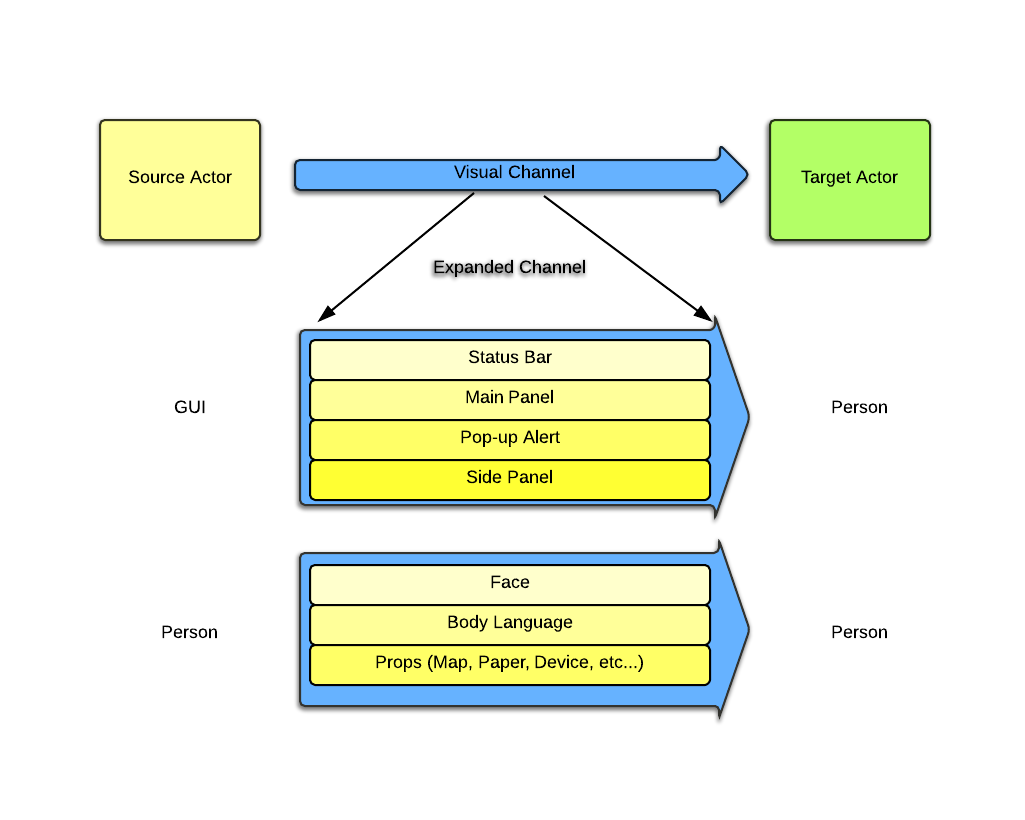
\includegraphics[width=6in]{layers.png}
\caption{Communication Channel Layers}
\label{fig:layers}
\end{center}
\end{figure}

We believe that this concept of channel layers creates a more natural flow of information across the DiTG while aligning the Model Abstraction Framework with modern human workload theory.  Additionally we have the ability to perform a number of different measurements on the channel layers that may prove valuable in obtaining accurate human workload measurements when combined with our other metrics.

